\documentclass{article}
\usepackage[spanish]{babel}
\usepackage[pdftex]{graphicx,color} 
\usepackage[utf8]{inputenc}
\usepackage{listings}
\usepackage{colortbl}
\usepackage{textcomp}
\usepackage{listings}
\usepackage{color}
\usepackage{wrapfig}
\usepackage{amsfonts}
\usepackage{amssymb}
\usepackage{algorithmic}
\usepackage{algorithm}
\usepackage[export]{adjustbox}
%\usepackage{amslatex}
\definecolor{lbcolor}{rgb}{0.9,0.9,0.9}
\lstset{
        backgroundcolor=, %\color{lbcolor},
        tabsize=4,
        rulecolor=,
        language=C,
        basicstyle=\scriptsize,
        upquote=true,
        aboveskip={1.5\baselineskip},
        %columns=fixed,
        showstringspaces=false,
        extendedchars=true,
        breaklines=true,
        prebreak = \raisebox{0ex}[0ex][0ex]{\ensuremath{\hookleftarrow}},
        frame=single,
        showtabs=false,
        showspaces=false,
        showstringspaces=false,
        identifierstyle=\ttfamily,
        keywordstyle=\color[rgb]{0,0,1},
        commentstyle=\color[rgb]{0.133,0.545,0.133},
        stringstyle=\color[rgb]{0.627,0.126,0.941},
	literate={á}{{\'a}}1
	{ã}{{\~a}}1
	{é}{{\'e}}1
	{ó}{{\'o}}1
	{í}{{\'i}}1
	{ñ}{{\~n}}1
	{¡}{{!`}}1
	{¿}{{?`}}1
	{ú}{{\'u}}1
	{Í}{{\'I}}1
	{Ó}{{\'O}}1
}

\topmargin -0.5in
\textwidth 6.8in
\textheight 9.0in
\oddsidemargin 0.0in
\evensidemargin 0.0in

\usepackage{enumitem}
\usepackage{multirow}
\usepackage{hhline}
\usepackage{multicol}
%ointpoints{punto}{puntos}

\begin{document}
\vspace{.5pc}
\centerline{\sc Clase Activa 4}
\centerline{\sc ELO320 - Estructura de Datos y Algoritmos}
\centerline{\sc Prof. Nicolás Gálvez Ramírez}
\vspace{2pc}
%\noindent {\bf Instrucciones}:
%\begin{itemize}
%    \item Conteste cada pregunta en una hoja separada. Éstas serán entregadas de tal forma al finalizar el certamen.
%    \item Si decide no contestar una pregunta, debe entregar una hoja sin respuestas en su lugar. 
%    \item Rotule claramente cada una de sus hojas con su Nombre Completo, Rol USM y Número de Paralelo.
%    \item El certamen tiene una duración de 60 minutos.
%\end{itemize}

%\noindent {\bf Preguntas}
%\medskip
\begin{itemize}

\begin{minipage}[h]{0.45\textwidth}
\item \textbf{Taxonomía de la memoria}. Rellene con su apunte a qué corresponde cada memoria y que tipo de elementos se almacenan en ellas.
\begin{enumerate}
\item text: 
\item static:
\item heap:
\item stack: 
\end{enumerate} 
\begin{center}
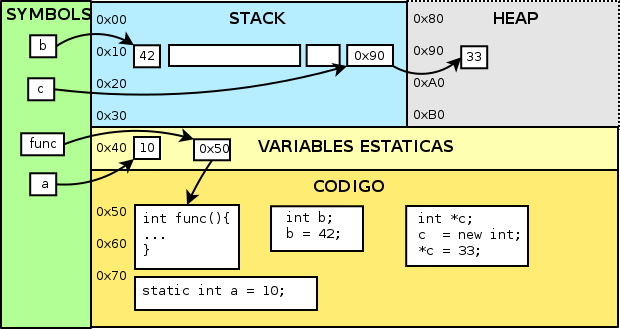
\includegraphics[width=.95\linewidth]{../images/progmemoria}
\end{center}
\end{minipage}
\hspace{0.5cm}
\begin{minipage}[h]{0.45\textwidth}
\item \textbf{Punteros}: Variables que almacenan direcciones de memoria. Se dice que apuntan a un tipo de dato, ya que en la dirección de memoria que almacenan se encuentra el tipo de dato especificado en su declaración.
\begin{lstlisting}[language=C, basicstyle=\scriptsize, escapeinside={|}{|}]
int main(){
	int utfsm1 = 1680; //Dos variables de tipo int.
	int utfsm2 = 3939; 
	
	int *dir = NULL;
	dir = &utfsm1; //Puntero a un int, apunta a donde está utfsm1
	
	printf("Dirección dentro de dir: |\%|p\n", dir);
	printf("Valor dir: |\%|d\n", *dir);
	printf("Dirección de dir: |\%|p\n", &dir);

	return 0;
}
\end{lstlisting}
\item \textbf{Operador \&} $\rightarrow$ Referencia o < <\textit{Dirección de memoria de}> >.
\item \textbf{Operador *} $\rightarrow$ Desreferencia o <<\textit{Ir a airección de memoria}> >. 
\end{minipage}

\begin{minipage}[h]{0.45\textwidth}
\item \textbf{Diferencias entre declaración con * y operador *}:
\begin{lstlisting}[language=C, basicstyle=\scriptsize, escapeinside={|}{|}]
int main(){
	float b = 1.0; 
	float * ptr; // * de declaración, solo indicamos que ptr
		     // almacena una dirección de memoria de un float
	
	ptr = &b; // sin *, modificamos la direccion a la que apunta ptr. 
	
	*ptr = 5.0; // * de desreferencia, se cambia el valor guardado 
		    // en la dirección de memoria apuntada por ptr
	
	b = *ptr + 1.0; // * de desreferencia, lo que hay guardado donde se apunta + 1.0 
	
	float * ptr2 = ptr; // * de declaración. 
}
\end{lstlisting}

\end{minipage}
\hspace{0.5cm}
\begin{minipage}[h]{0.45\textwidth}
\item \textbf{Aritmética de Punteros}: Las direcciones que guardan los punteros varían segun el peso del tipo de dato apuntado. Así se transforma 1 unidad decimal en 1 unidad segun el tamaño del tipo.
\begin{lstlisting}[language=C, basicstyle=\scriptsize, escapeinside={|}{|}]
int main(){
	float num = 2.5;
	float *f;
	f = &num; //Dirección a num.

	printf("Direccion f: |\%|p\n", f); //¿Cuál es la diferencia
	printf("Direccion f+1: |\%|p\n", f+1); //entre f y f+1?
	// peso de 1 float -> 4 bytes en hexadecimal. 
}
\end{lstlisting}
\end{minipage}

\begin{minipage}[h]{0.45\textwidth}
\item \textbf{Aritmética de Punteros y Arreglos}: Los punteros son compatibles con los arreglos (no son lo mismo), así que podemos recorrer un arreglo con esta alternativa. 
\begin{lstlisting}[language=C, basicstyle=\scriptsize, escapeinside={|}{|}]
int main(){
	int a[10], i;
	int *pa, *pb;
	pa = &a[0]; /* dir. elemento 0 de arreglo a. tamaño 1 int */
	pa = a;	    /* hace lo mismo que la linea anterior con coerción */
	pb = &a;    /* dir. de arreglo a. tamaño 10 int */
	
	for (i=0; i<10; i++){ //tres formas de recorrer
		printf("|\%|d ", a[i]);
		printf("|\%|d ", *(pa+i));
		printf("|\%|d ", *(a+i));
	}
	
	printf(printf("|\%|d ", *(pb+1)); //¿Qué pasa acá?
}
\end{lstlisting}

\end{minipage}


\begin{minipage}[h]{0.45\textwidth}
\item \textbf{Paso por Valor}: Los parametros, que son variables locales, copian los valores que fueron pasados como parámetros. Las variables originales se mantienen inalteradas.
\begin{lstlisting}[language=C, basicstyle=\scriptsize, escapeinside={|}{|}]
#include<stdio.h>

void swap(int a, int b){
	int temp;
	temp = a;
	a = b;
	b = temp;
}

int main(){
	int x=2, y=3;
	swap(x,y);
	printf("x: |\%|d, y: |\%|d\n", x, y); //¿Qué imprime?
	return 0;
}
\end{lstlisting}
\end{minipage}
\hspace{0.5cm}
\begin{minipage}[h]{0.45\textwidth}
\item \textbf{Paso por referencia}: Los parámetros pasan a ser punteros locales, copiando la dirección de memoria de un elemento. Se hace derreferencia, y así se modifica las variables originales de forma indirecta (un puntero apuntando a ellas).
\begin{lstlisting}[language=C, basicstyle=\scriptsize, escapeinside={|}{|}]
#include<stdio.h>

void swap(int *a, int *b){ //punteros locales
	int temp;
	temp = *a; //se guarda lo que hay donde apunta a
	*a = *b; //cambio entre los valores donde apuntan los punteros
	*b = temp; //agrego valor guardado, no se cambian los punteros, ojo.
}

int main(){
	int x=2, y=3;
	swap(|\&|x,|\&|y);
	printf("x: |\%|d, y: |\%|d\n", x, y); //¿Qué imprime?
	return 0;
}
\end{lstlisting}
\end{minipage}


\end{itemize}
\end{document}

